\documentclass[a4paper,11pt]{article}
\usepackage[T1]{fontenc}
\usepackage[utf8]{inputenc}
\usepackage{lmodern}

\title{Neural network notes}
\author{Marco Marini}

\begin{document}

\maketitle
\tableofcontents

\begin{abstract}
Studio del gioco wall
\end{abstract}

\section{Generale}

Wall è un gioco dove una pallina si muove in un campo rettangolare con traiettorie rettilinee diagonali.
I limiti superiore e laterali sono costituiti da muri che
fanno rimbalzare la pallina.
La parte inferiore invece è aperta e una paletta controllata
da giocatore si muove orizzontalmente permettendo allo stesso di far rimbalzare la pallina all'interno del campo da 
gioco.

$
\begin{array}{ccccccccccccccc}
=	& = & = & = & = & = & = & = & = & = & = & = & = & = & = \\
|	&  &  &  &  &  &  &  &  &  &  &  &  &  & | \\ 
|	&  &  &  &  &  &  &  &  &  &  &  &  &  & | \\ 
|	&  &  &  &  &  &  &  &  &  &  &  &  &  & | \\ 
|	&  &  &  &  &  &  &  &  &  &  &  &  &  & | \\ 
|	&  &  &  &  &  &  &  &  &  &  &  &  &  & | \\ 
|	&  &  &  &  &  & O &  &  &  &  &  &  &  & | \\ 
|	&  &  &  &  &  &  &  &  &  &  &  &  &  & | \\ 
|	&  &  &  &  &  &  &  &  &  &  &  &  &  & | \\ 
|	&  &  &  &  &  &  &  &  &  &  &  &  &  & | \\ 
	&  &  & = & = & = &  &  &  &  &  &  &  &  & 
\end{array} 
$

Definiamo 
\[ n = 10 \] il numero di righe del campo
\[ m = 13 \] il numero di colonne
\[ w = 3 \] la larghezza della paletta


\section{Spazio degli stati}
In un qualsiasi momento lo stato del gioco è rappresentato dalla posizione
della pallina, la direzione di spostamento della pallina e la posizione della paletta.
Calcoliamo il numero di stati possibili:

La paletta può trovarsi in uno degli
\[m - w + 1 = 8\] possibili posizioni.

Quando la pallina non si trova n prossimtà dei muri o della paletta
può muoversi in 4 diverse direzioni: NE, SE, SO, NO.
Quindi abbiamo
\[ 4 (n-2)(m-2) (m - w + 1) = 2816 \]
possibili stati della pallina.

Negli angoli superiori la pallina può avere solo una direzione quindi
si aggiungono altri 
\[
	2 (m -w +1) = 16
\] stati.

Quando si trova in prossimità invece del muro superiore o di quelli laterali, la pallina può assumere solo due possibili velocità quindi avremo:
\[ (m -w + 1) 2 [ 2 (n - 2) + m - 2] = 432 \]
ulteriori stati.

Vediamo ora alcuni particolari quando la pallina si trova su nell'angolo
inferiore sx nel qual caso è possibile una sola traiettoria verso l'alto
se la paletta si trova in prima o seconda posizione (rimbalzo) o verso 
l'uscita del campo negli altri casi, quindi avremo
\[ m-w+1 = 8\] possibili casi.

Altrettanti se consideriamo quando la pallina si trova nell'angolo inferiore dx.

Nel caso invece la pallina si trovi sulla riga inferiore del campo avremo due possibili traiettorie: NE o  NO se la pallina si trova esattamente sotto la paletta (rimbalzo) o SE o SO negli altri casi.
\begin{figure}
\centering
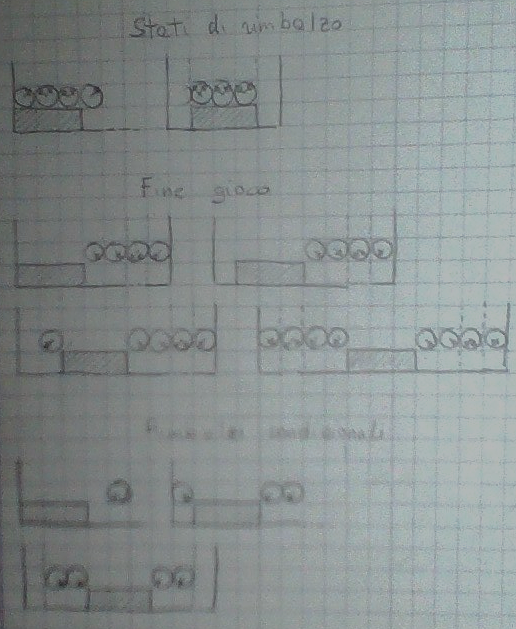
\includegraphics[width=0.7\linewidth]{wall1}
\caption{}
\label{fig:wall1}
\end{figure}

Quindi avremo
\[ 2 * (m - 2) = 16 \] stati.

Poi avremo lo stato finale di pallina fuori campo.

In totale quindi possiamo contare
\[
	2816 + 16 + 432 + 8 + 8 + 16 + 1 = 3297
\] possibili stati.





\end{document}
